\documentclass{article}

% if you need to pass options to natbib, use, e.g.:
%     \PassOptionsToPackage{numbers, compress}{natbib}
% before loading neurips_2018

% ready for submission
% \usepackage{neurips_2018}

% to compile a preprint version, e.g., for submission to arXiv, add add the
% [preprint] option:
%     \usepackage[preprint]{neurips_2018}

% to compile a camera-ready version, add the [final] option, e.g.:
\usepackage[preprint]{neurips_2018}

% to avoid loading the natbib package, add option nonatbib:
%     \usepackage[nonatbib]{neurips_2018}

\usepackage[utf8]{inputenc} % allow utf-8 input
\usepackage[T1]{fontenc}    % use 8-bit T1 fonts
\usepackage{hyperref}       % hyperlinks
\usepackage{url}            % simple URL typesetting
\usepackage{booktabs}       % professional-quality tables
\usepackage{amsfonts}       % blackboard math symbols
\usepackage{microtype}      % microtypography
\usepackage{graphicx}
\usepackage{float}

\title{Bandit networks}

% The \author macro works with any number of authors. There are two commands
% used to separate the names and addresses of multiple authors: \And and \AND.
%
% Using \And between authors leaves it to LaTeX to determine where to break the
% lines. Using \AND forces a line break at that point. So, if LaTeX puts 3 of 4
% authors names on the first line, and the last on the second line, try using
% \AND instead of \And before the third author name.

\author{%
  Charles \textsc{Auguste} \\
  École des Ponts \\
  \texttt{charles.auguste@ponts.org} \\
  \And
  Louis \textsc{Trezzini} \\
  École des Ponts \\
  \texttt{louis.trezzini@ponts.org} \\
}

\begin{document}

\maketitle

\begin{abstract}
  A single-agent multi-armed bandit (MAB) problem is a problem in which a gambler, being in face of several slot machines, has to decide which machines to play, how many times and in which order to play each machine.
  % There are two different goals in such problems, regret minimization which aims at maximizing the total reward along the trials, and best arm identification which aims at identifying as quickly as possible the best arm. In this project we will mainly focus on the first aspect.
  In this project, we consider a multi-agent MAB scenario in which a group of agents connected through a social network are engaged in playing a stochastic MAB game and focus on minimizing their regret. Every time a player takes an action, the reward is observed by both the agent and its neighbors in the network.
  The goal of this project is to understand different collaborative policies (NAIC-type and FYL) described in \cite{DBLP:journals/corr/KollaJG16}, and to compare their performance over different network structures.
\end{abstract}

\section{Introduction}


\section{...}


\section{Theoretical contributions}

%FIXME

\newpage

\section{Experimental results}

\subsection{Reproducing experiments from \cite{DBLP:journals/corr/KollaJG16}}

\subsubsection{Experiment 1}

Performance comparison of UCB-Network policy on various 10 node networks: 2 arms, Bernoulli rewards with means $0.5$ and $0.7$.

\begin{figure}[H]
  \centering
  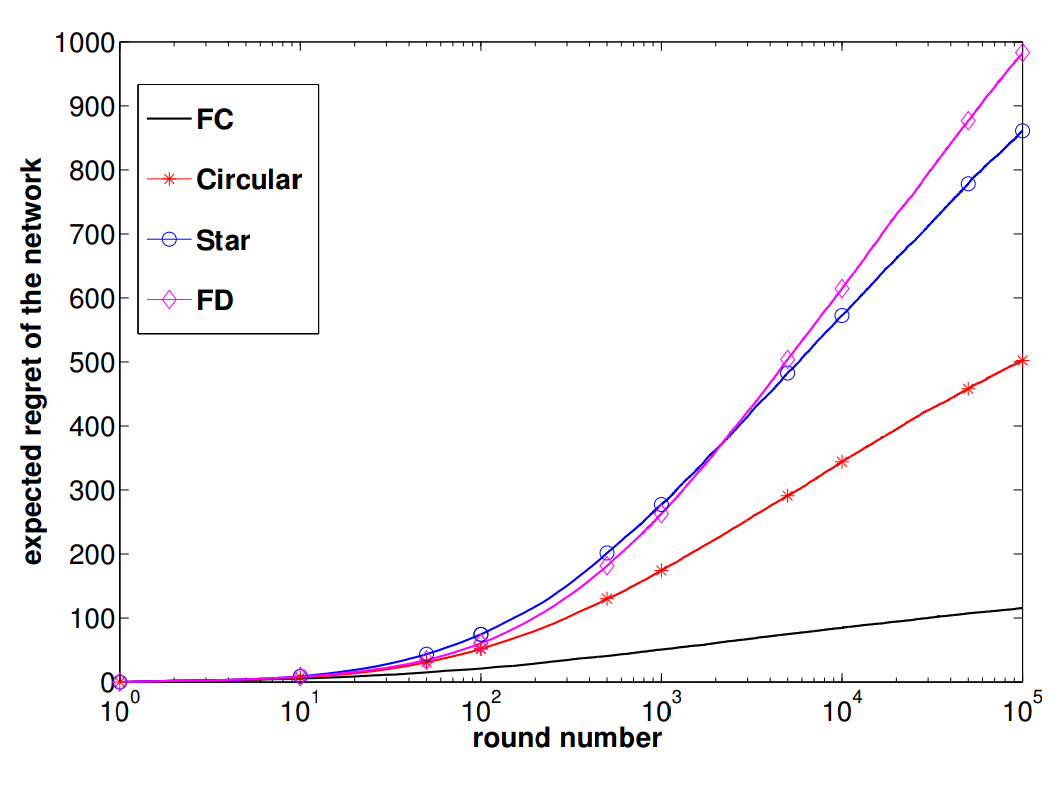
\includegraphics[width=0.49\linewidth]{fig1_1.png}
  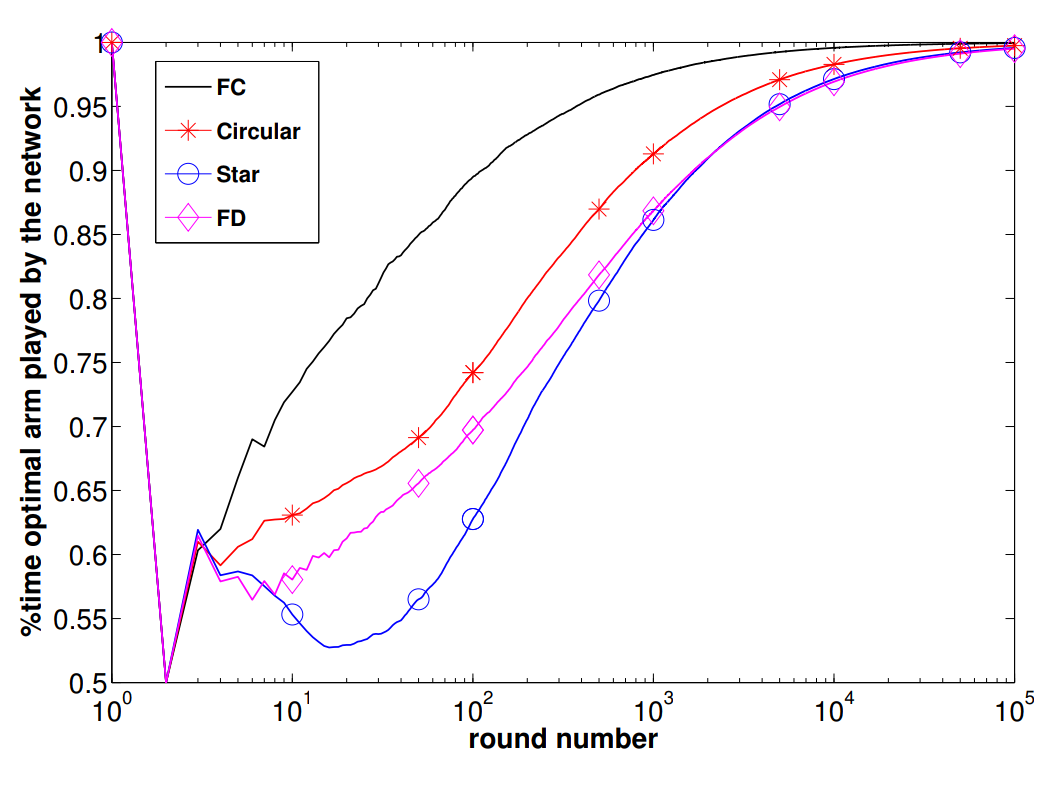
\includegraphics[width=0.49\linewidth]{fig1_2.png}
  \caption{Results for experiment 1 from \cite{DBLP:journals/corr/KollaJG16} (100 sample paths).}
\end{figure}

\begin{figure}[H]
  \centering
  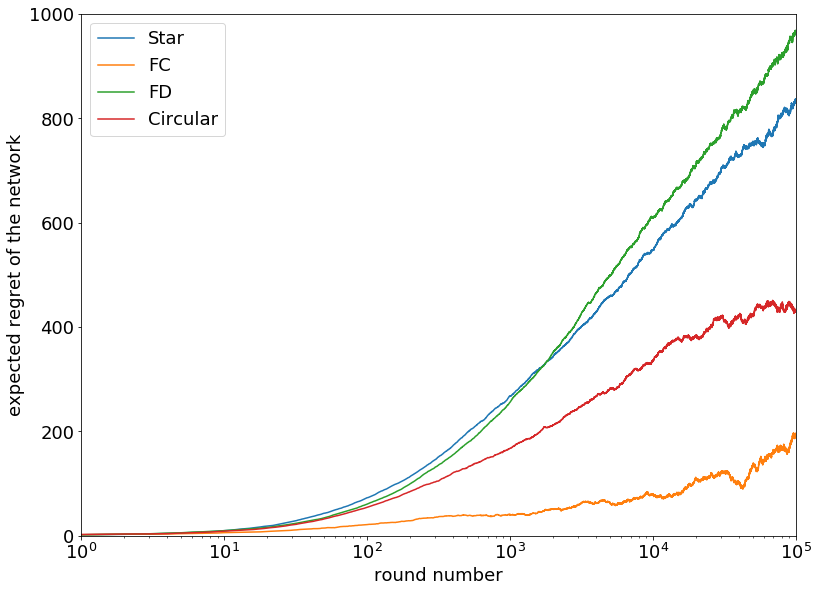
\includegraphics[height=5cm]{fig1_1_ours.png}
  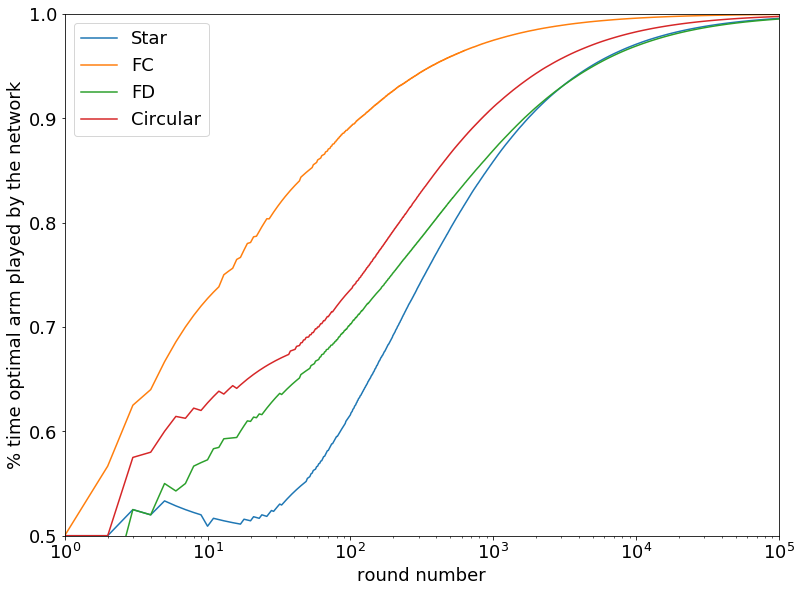
\includegraphics[height=5cm]{fig1_2_ours.png}
  \caption{Our results for experiment 1 (1000 sample paths).}
\end{figure}

\subsubsection{Experiment 2}

Performance comparison of UCB-Network policy on various 20 node networks: 10 arms, Bernoulli rewards with means $0.1, 0.2, \dots, 1$.

\begin{figure}[H]
  \centering
  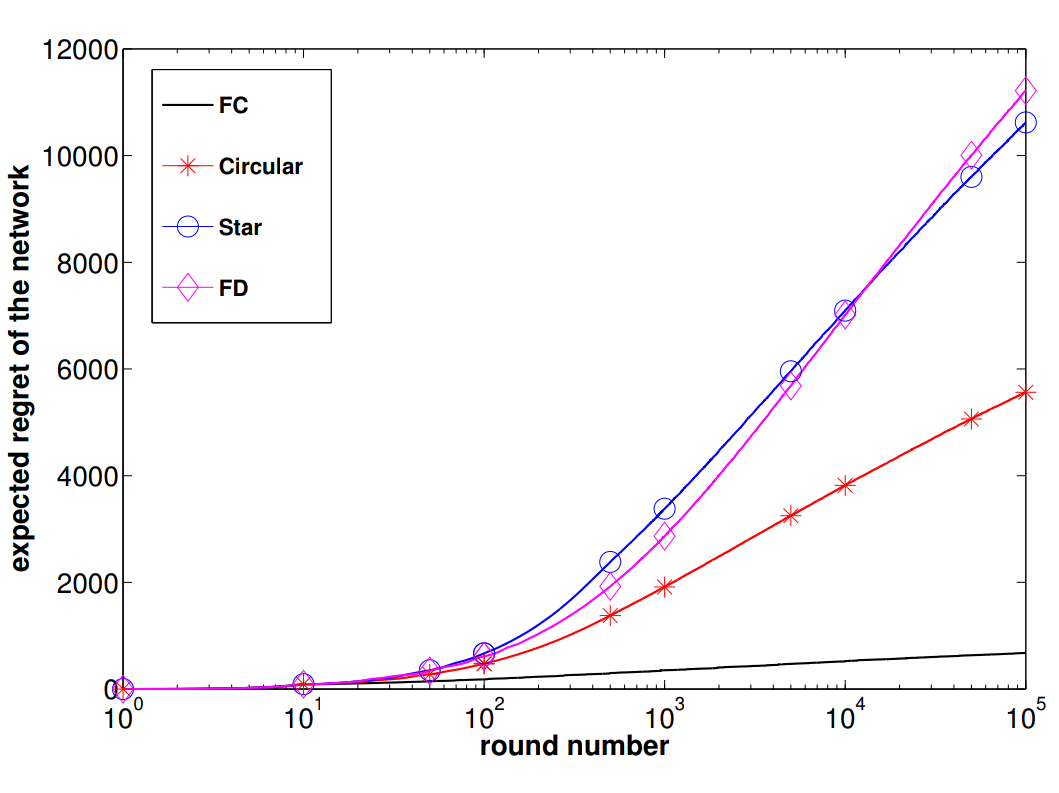
\includegraphics[width=0.49\linewidth]{fig2_1.png}
  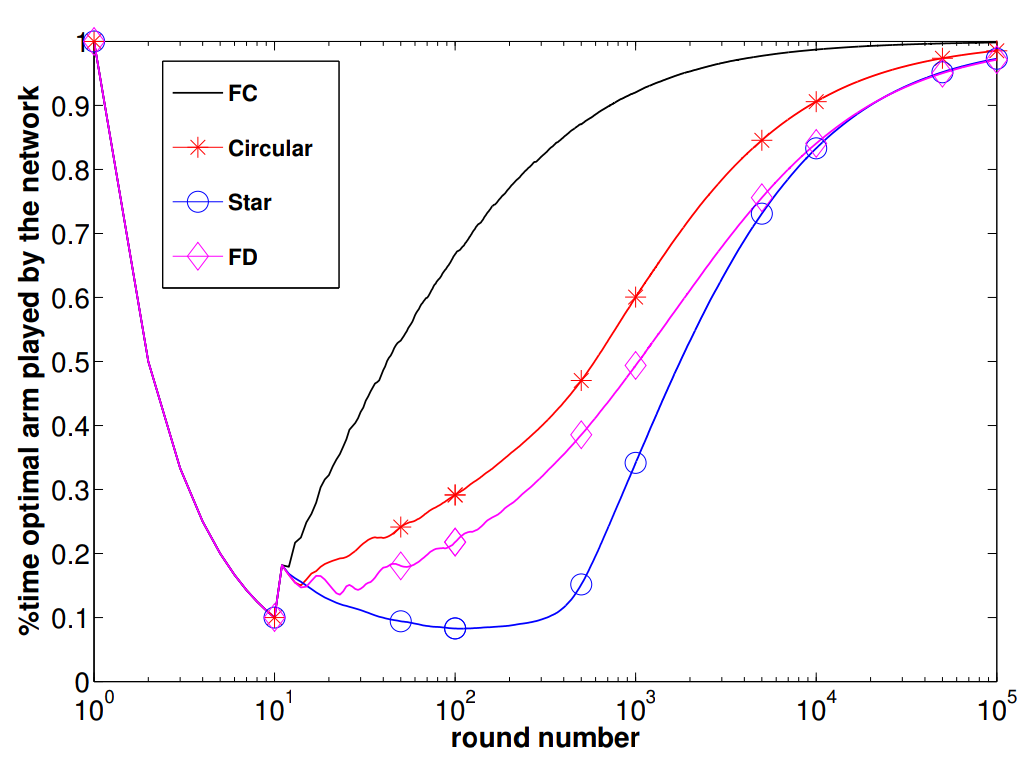
\includegraphics[width=0.49\linewidth]{fig2_2.png}
  \caption{Results for experiment 2 from \cite{DBLP:journals/corr/KollaJG16} (100 sample paths).}
\end{figure}

\begin{figure}[H]
  \centering
  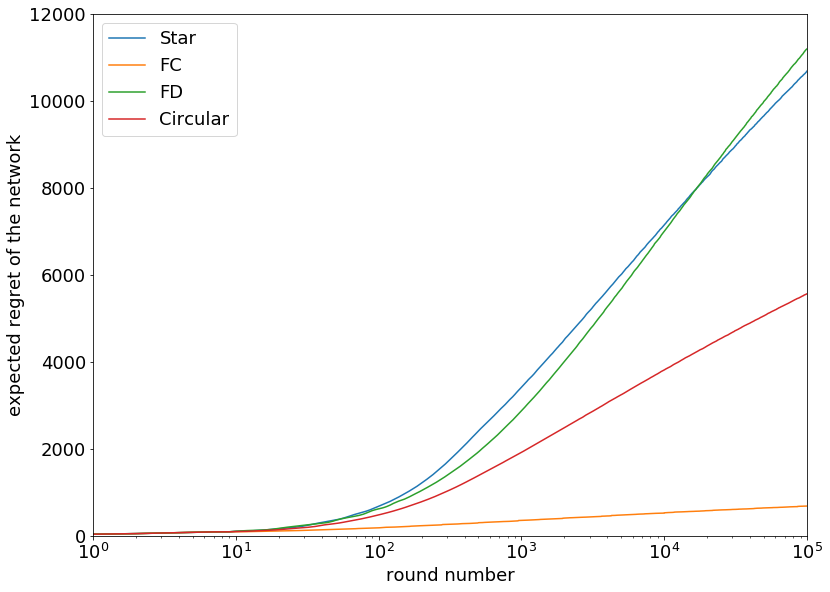
\includegraphics[width=0.49\linewidth]{fig2_1_ours.png}
  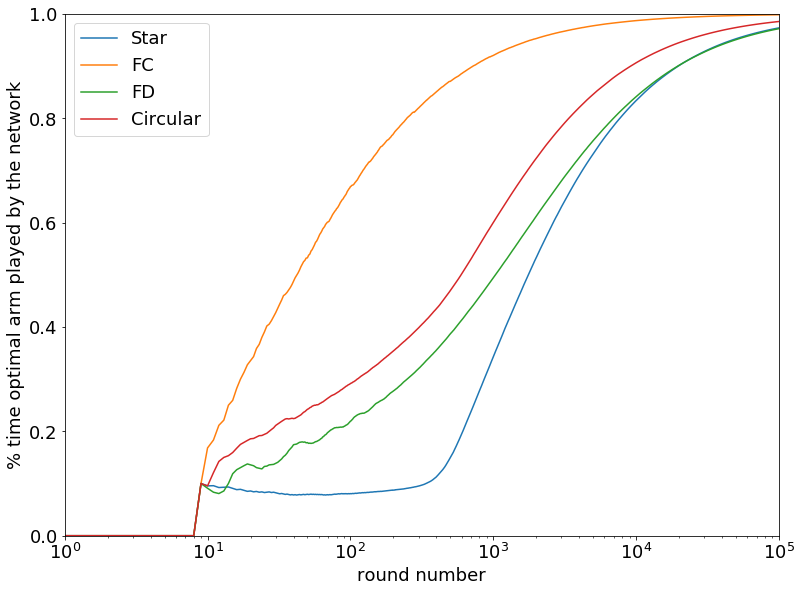
\includegraphics[width=0.49\linewidth]{fig2_2_ours.png}
  \caption{Our results for experiment 2 (1000 sample paths).}
\end{figure}

\subsubsection{Experiment 3}

Performance comparison of UCB-Network and FYL policies on various star networks: 2 arms, Bernoulli rewards with means $0.5$ and $0.7$.

\begin{figure}[H]
  \centering
  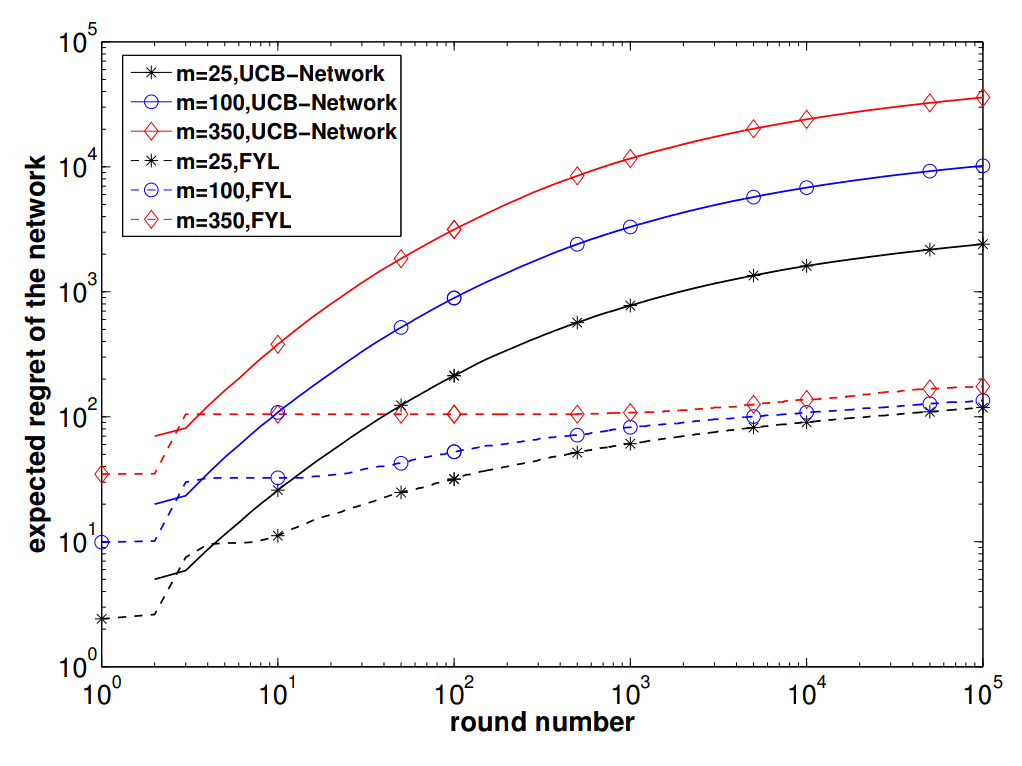
\includegraphics[width=0.49\linewidth]{fig3_1.png}
  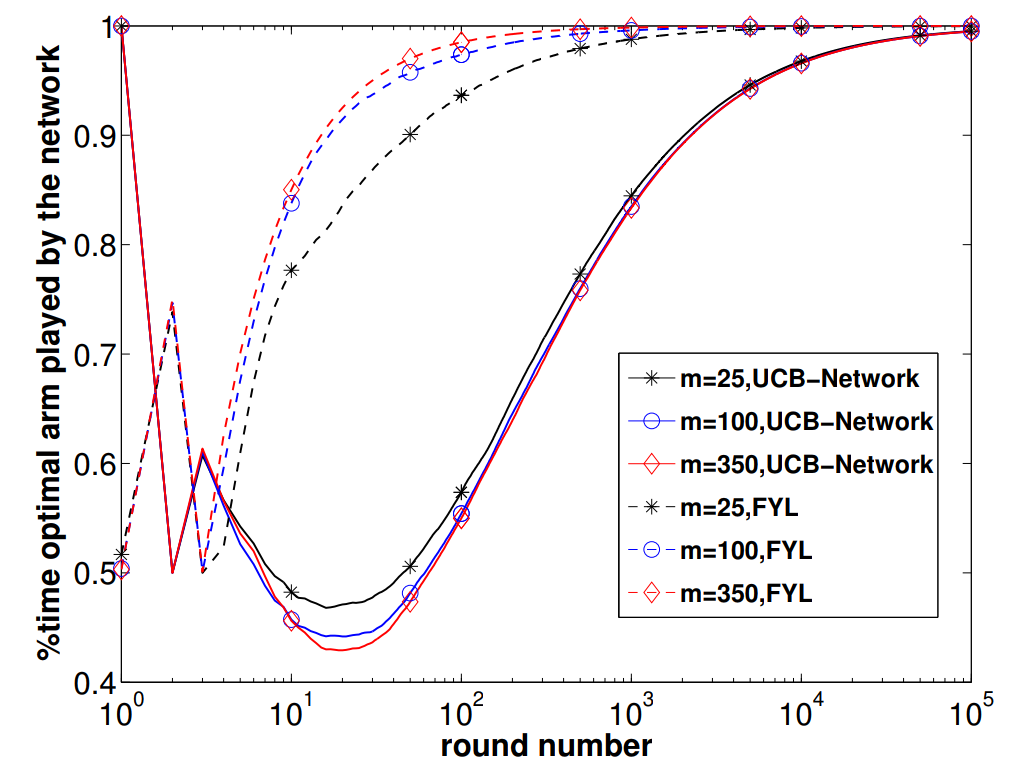
\includegraphics[width=0.49\linewidth]{fig3_2.png}
  \caption{Results for experiment 3 from \cite{DBLP:journals/corr/KollaJG16} (100 sample paths).}
\end{figure}

\begin{figure}[H]
  \centering
  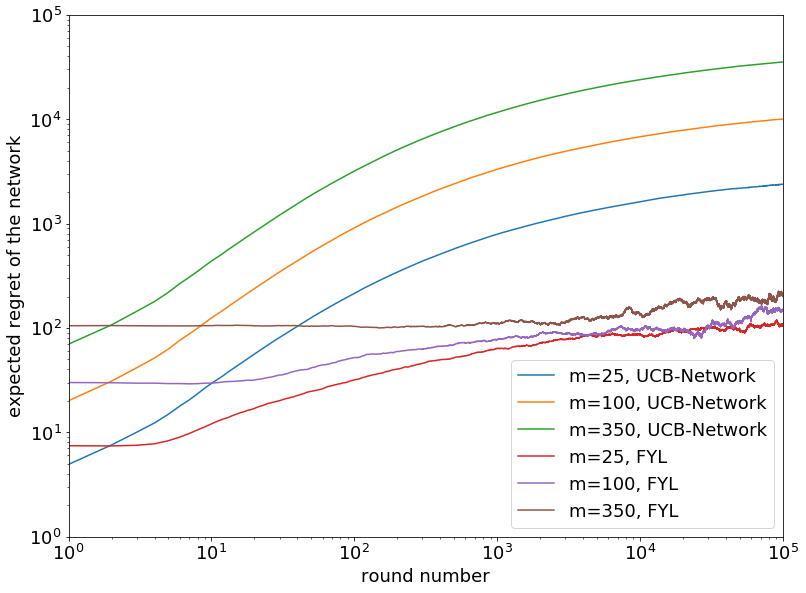
\includegraphics[width=0.49\linewidth]{fig3_1_ours.png}
  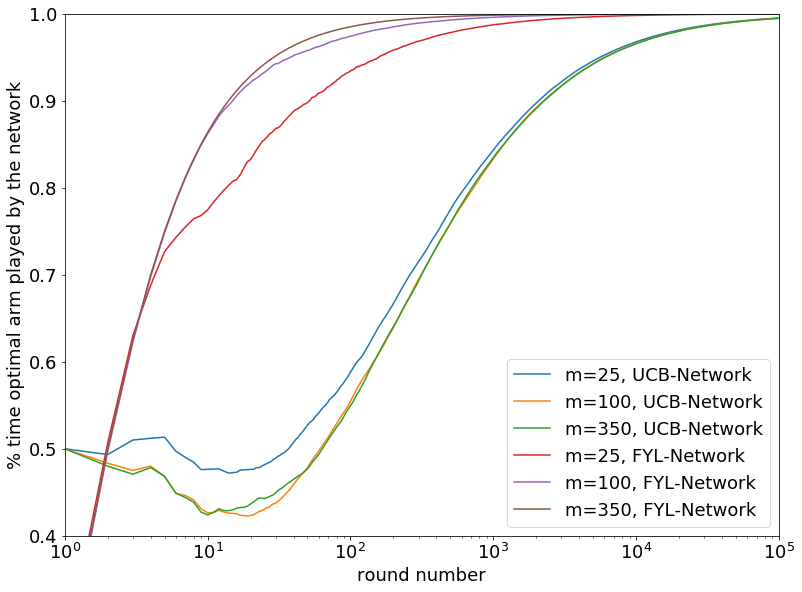
\includegraphics[width=0.49\linewidth]{fig3_2_ours.png}
  \caption{Our results for experiment 3 (1000 sample paths).}
\end{figure}

\subsection{Distributed star network}



\section{Conclusion}

{\small
\bibliographystyle{unsrt}
\bibliography{biblio}
}

% FIXME remove everything below
\newpage

\section{Citations, figures, tables, references}
\label{others}

These instructions apply to everyone.

\subsection{Citations within the text}

The \verb+natbib+ package will be loaded for you by default.  Citations may be
author/year or numeric, as long as you maintain internal consistency.  As to the
format of the references themselves, any style is acceptable as long as it is
used consistently.

The documentation for \verb+natbib+ may be found at
\begin{center}
  \url{http://mirrors.ctan.org/macros/latex/contrib/natbib/natnotes.pdf}
\end{center}
Of note is the command \verb+\citet+, which produces citations appropriate for
use in inline text.  For example,
\begin{verbatim}
   \citet{hasselmo} investigated\dots
\end{verbatim}
produces
\begin{quote}
  Hasselmo, et al.\ (1995) investigated\dots
\end{quote}

If you wish to load the \verb+natbib+ package with options, you may add the
following before loading the \verb+neurips_2018+ package:
\begin{verbatim}
   \PassOptionsToPackage{options}{natbib}
\end{verbatim}

If \verb+natbib+ clashes with another package you load, you can add the optional
argument \verb+nonatbib+ when loading the style file:
\begin{verbatim}
   \usepackage[nonatbib]{neurips_2018}
\end{verbatim}

As submission is double blind, refer to your own published work in the third
person. That is, use ``In the previous work of Jones et al.\ [4],'' not ``In our
previous work [4].'' If you cite your other papers that are not widely available
(e.g., a journal paper under review), use anonymous author names in the
citation, e.g., an author of the form ``A.\ Anonymous.''

\subsection{Tables}

All tables must be centered, neat, clean and legible.  The table number and
title always appear before the table.  See Table~\ref{sample-table}.

Place one line space before the table title, one line space after the
table title, and one line space after the table. The table title must
be lower case (except for first word and proper nouns); tables are
numbered consecutively.

Note that publication-quality tables \emph{do not contain vertical rules.} We
strongly suggest the use of the \verb+booktabs+ package, which allows for
typesetting high-quality, professional tables:
\begin{center}
  \url{https://www.ctan.org/pkg/booktabs}
\end{center}
This package was used to typeset Table~\ref{sample-table}.

\begin{table}
  \caption{Sample table title}
  \label{sample-table}
  \centering
  \begin{tabular}{lll}
    \toprule
    \multicolumn{2}{c}{Part}                   \\
    \cmidrule(r){1-2}
    Name     & Description     & Size ($\mu$m) \\
    \midrule
    Dendrite & Input terminal  & $\sim$100     \\
    Axon     & Output terminal & $\sim$10      \\
    Soma     & Cell body       & up to $10^6$  \\
    \bottomrule
  \end{tabular}
\end{table}

\end{document}
